\chapter{Future Work} \label{chap:fw}

\section{Further datasets}
The datasets that used in this dissertation are relatively small---on the order of 10s of different parameter combinations.
The limited scope of these datasets means that they are only able to coarsely cover the entire parameter space.
I hypothesize that one way to get better reduced models would be to train using data generated from more of the parameter space.
Generating large biological datasets by hand is difficult and error prone.
However, this dissertation demonstrated the potential for further lab automation by generating a dataset using the Labcyte Echo liquid handler.
Future work will take this even further and generate datasets with hundreds or even thousands of starting conditions.
Another logical extension is to use datasets generated from organisms other than \gls{ecoli}.

\begin{figure}[t!]
\begin{center}
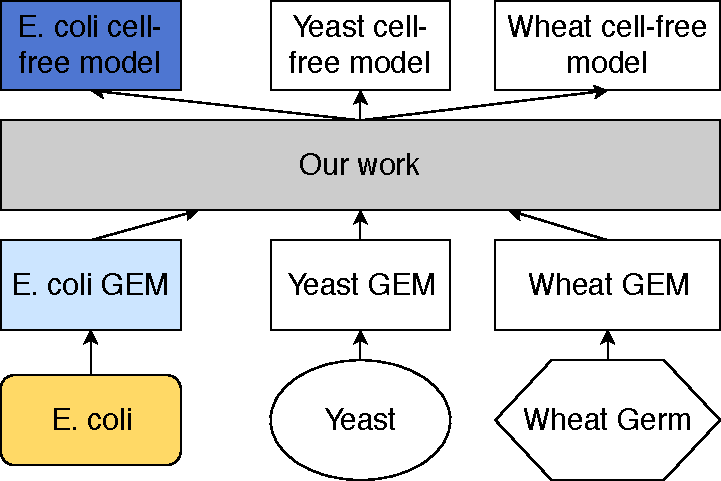
\includegraphics{figs/Vision.pdf}
\caption[\gls{sys} can generate cell-free models for any organism]
{\gls{sys} was designed to convert any organism's \glspl{gem} into an appropriate cell-free model.
}
\end{center}
\label{fig:vision}
\end{figure}

\section{Different Organisms}
This work has only explored the generation of \gls{ecoli} cell-free models.
However, much ongoing work involves the use of non-\gls{ecoli} organisms.
This system was written in such a way that it can be applied to any organism with a \gls{gem}.
Figure \ref{fig:vision} demonstrates one potential vision of how \gls{sys} could be used in the future.
Instead of creating a model by hand that only describes our \gls{cfps} system, \gls{sys} can be used to create cell-free metabolic models for many different organisms.
In particular, I am also a part of an OpenPlant grant involving modeling wheat-germ cell-free systems.
The data is currently being generated, and I plan to apply \gls{sys} to this new \gls{cfps} system as soon possible.

%One issue is that this pipeline is only as good as the initial models.
%The initial \gls{fba} model is an imperfect description of a full \gls{ecoli} cell, so any errors in that overall model will be replicated in our reduced models.
%\gls{fba} models are periodically updated with new data.
%Our system is built to be flexible and can easily produce new models based on any updates.

\section{RL system for reduction}
The use of a \gls{vae} as a dimensionality reduction tool proved to be quite powerful, but the part of the system that converted from the reduced representation back into a \gls{fba} model was quite simple.
\gls{sys} removes reactions based on a simple thresholding criterion.
Instead of deciding which reactions to remove using a threshold, future version of \gls{sys} could reframe this problem as a reinforcement learning problem.
Using a combination of experimental data, a starting \gls{fba} model, and a latent representation of the problem space, these more sophisticated search methods could likely produce better reduced models.
To that end, I have also built a framework on top of OpenAI's Gym environment for performing reinforcement learning on \gls{fba} models.
Given a starting model with almost 2600 reactions, the search space of possible reduced models is enormous.
However, a combination of the Corr-VAE and reinforcement learning could perform a targeted search and yield a better reduced model.

\begin{figure}[t!]
\begin{center}
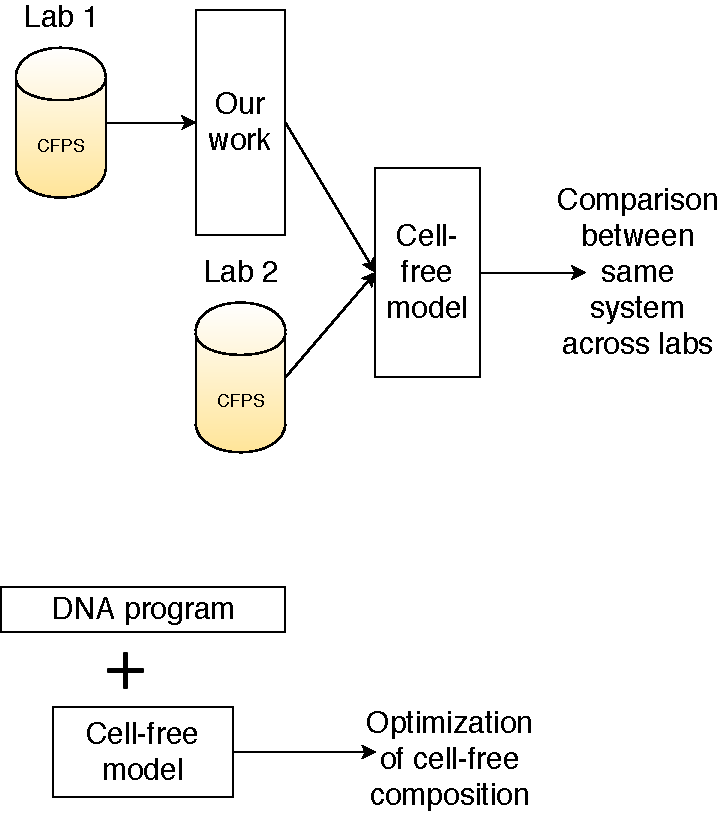
\includegraphics{figs/Applications.pdf}
\caption[Future applications of \gls{sys}]
{Two future applications of \gls{sys}.
Above, multiple experiments can be projected in the same subspace to better compare experimental results.
Below, the system can help optimize the energetic composition of a cell-free system}
\end{center}
\label{fig:apps}
\end{figure}

\section{Batch variation}
Finally, an important use case for \gls{sys} is as a way to deal with batch variation in \gls{cfps} systems.
Batch variation is an important problem facing the cell-free community~\cite{sun2013protocols, chizzolini2017cell}.
The current solution to this problem is to run everything that needs to be compared in the same batch.
This is problematic, though, if the batch runs out or someone else wants to reproduce this result.
The only way to deal with this problem would be to redo all of the experiments in a new batch.

Figure \ref{fig:apps} demonstrates how \gls{sys} provides a potential solution to this issue of batch variation.
A researcher runs a calibration set of experiments and then uses those experimental results to generate a \gls{vae} model.
Now, this \gls{vae} can be used to project any future experimental data into the same latent space as the first set of experiments.
These experiments could be compared within the latent space, or they could be transformed back into the original dimensionality of the data and then compared.
This transformed data should allow for better comparisons across batches.

% Generative nature of VAEs
% Can generate "typical" fluxes for a subspace
% Traverse the subspace 